\chapter{SYSTEM SCREENSHOTS AND DESCRIPTIONS}

\section{Introduction}
This chapter provides a visual walkthrough of the developed web application. It includes screenshots of the key user interfaces along with detailed descriptions of their specific functionalities within the context-aware presence verification system.

\section{Login Authentication Interface}
The login interface is the primary entry point to the system. It enforces Role-Based Access Control (RBAC), ensuring that Administrators, Special Members (such as the Principal or Director), and regular Staff only access the modules they are authorized for. The authentication is firmly secured using JSON Web Tokens (JWT).

\begin{figure}[H]
\centering
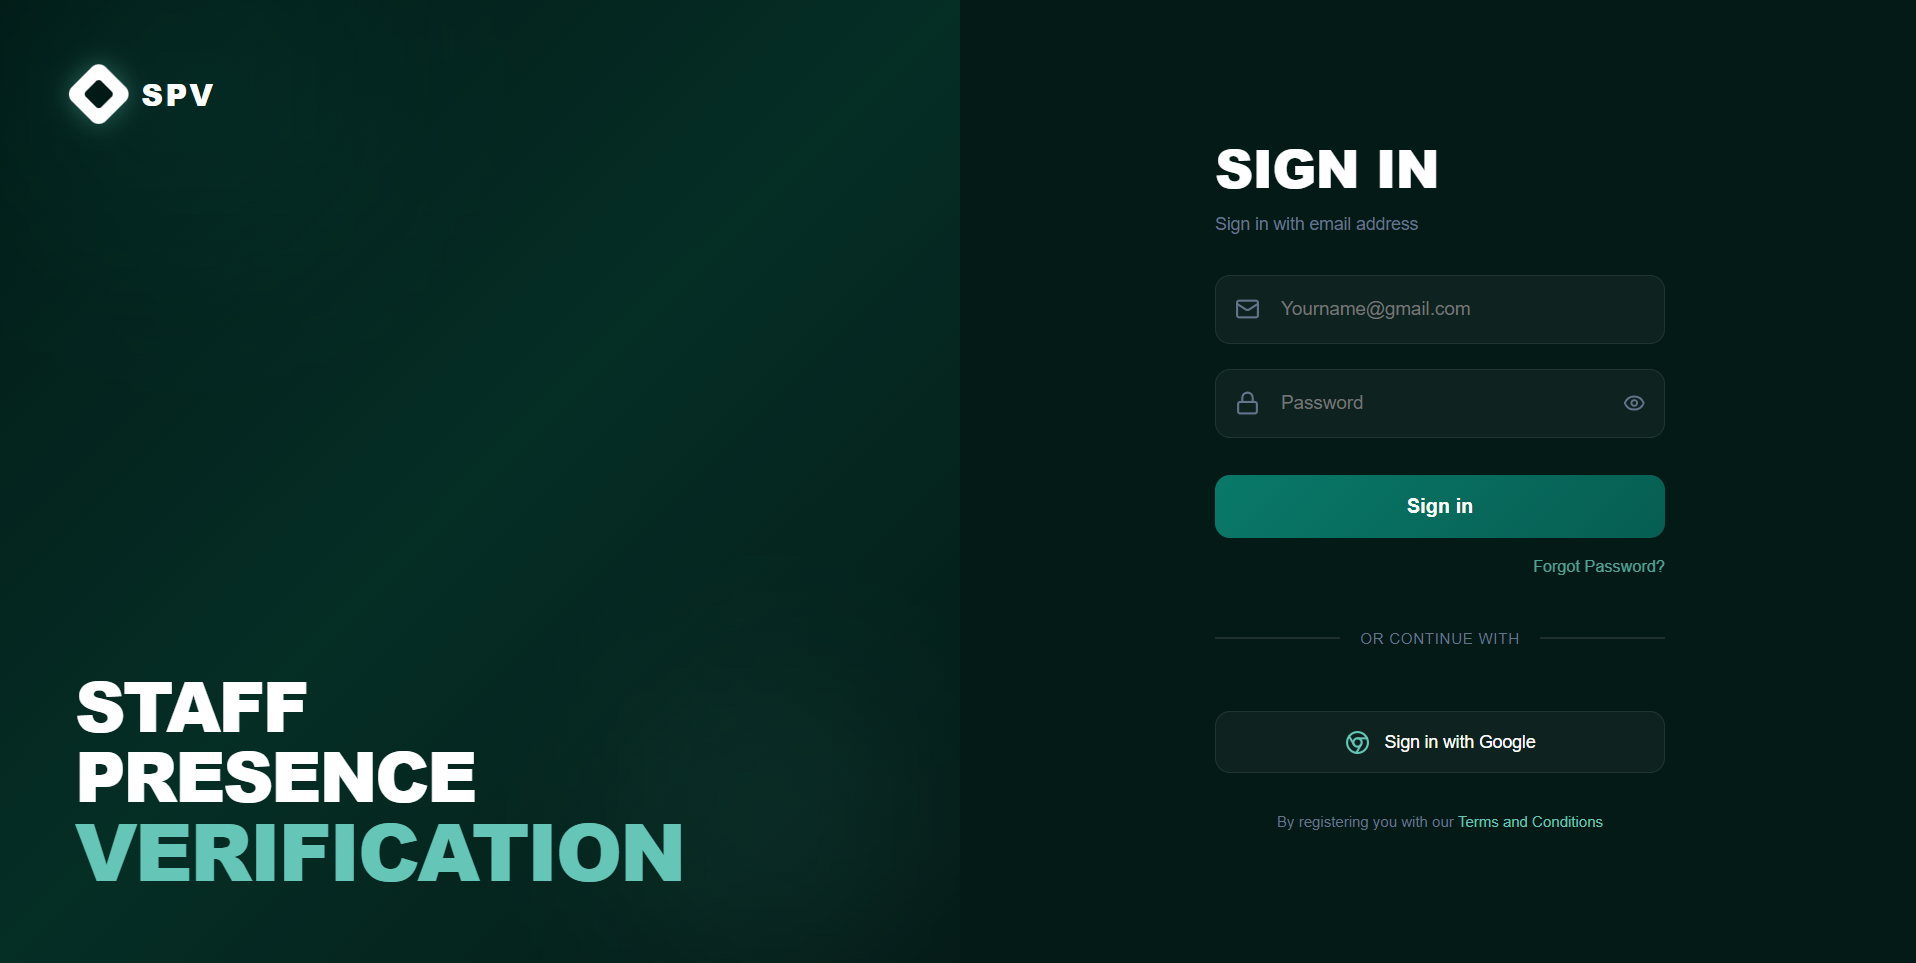
\includegraphics[width=0.8\textwidth]{images/login_page.png}
\caption{Login Authentication Interface}
\end{figure}

\section{Admin Live Tracking Dashboard}
The live tracking dashboard is the core monitoring tool. It continuously fetches proximity data processed by the ESP32 hardware receivers and compares it against the scheduled timetable engine. The dashboard dynamically categorizes staff into three distinct states based on the context:
\begin{itemize}
    \item \textbf{In-Class (Present)}: The staff member's BLE tag is verified physically in the correctly assigned room.
    \item \textbf{Absent or Left}: The staff member is scheduled for a class but not detected by any nearby ESP32 receiver.
    \item \textbf{On Leave}: The staff member has a pre-approved leave request stored in the database for the current day.
\end{itemize}

\begin{figure}[H]
\centering
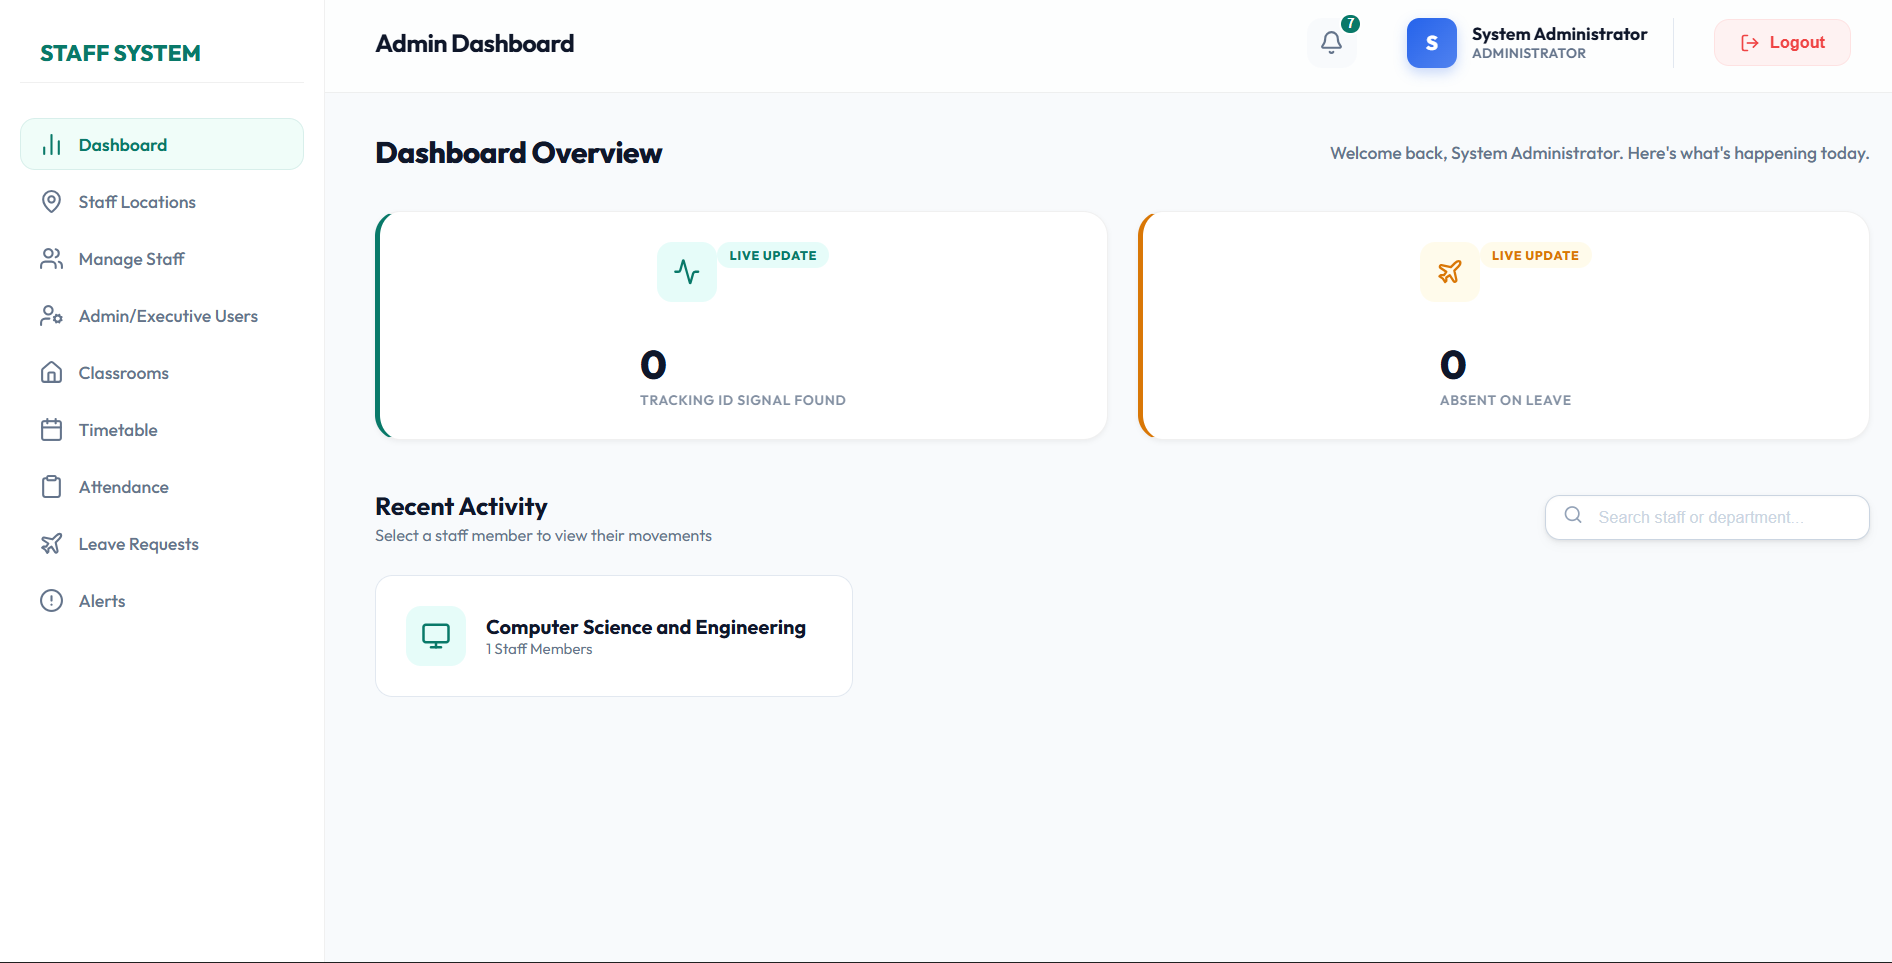
\includegraphics[width=0.8\textwidth]{images/admin_dashboard.png}
\caption{Administrator Real-Time Staff Status Dashboard}
\end{figure}

\section{Timetable Configuration Module}
This interface allows department heads and administrators to configure the weekly master timetable. It seamlessly maps a specific staff member to a subject branch, a physical classroom location, and a distinct day/time slot. This exact mapping is what enables the backend "Context-Aware" logic layer to algorithmically decide if a BLE detection represents a valid, legitimate work event.

\begin{figure}[H]
\centering
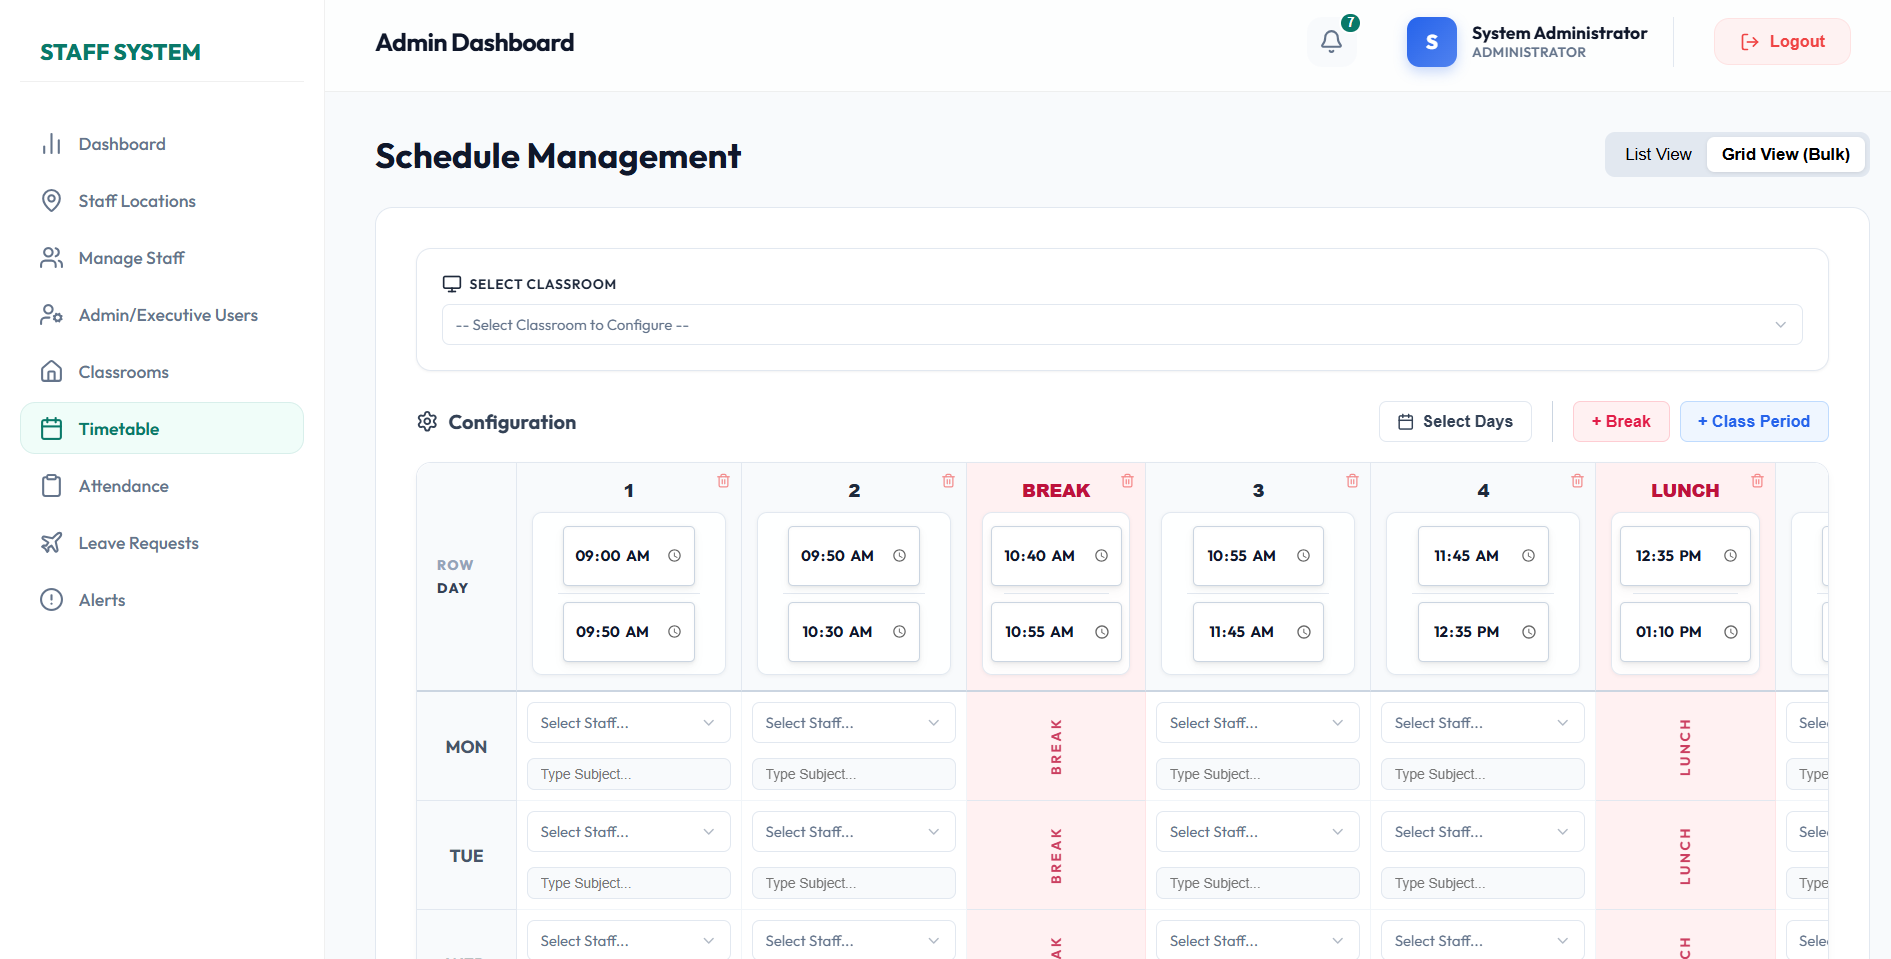
\includegraphics[width=0.8\textwidth]{images/timetable_manager.png}
\caption{Timetable Configuration and Assignment Module}
\end{figure}

\section{Automated Attendance Reports and Logs}
The reporting interface provides historical accounting data. Instead of relying on manual entry, the backend system automatically writes permanent logs when a staff member successfully passes the BLE verification filter for a scheduled class period. The admin can powerfully filter these logs by specific dates, individual staff IDs, and departments to export official attendance records.

\begin{figure}[H]
\centering
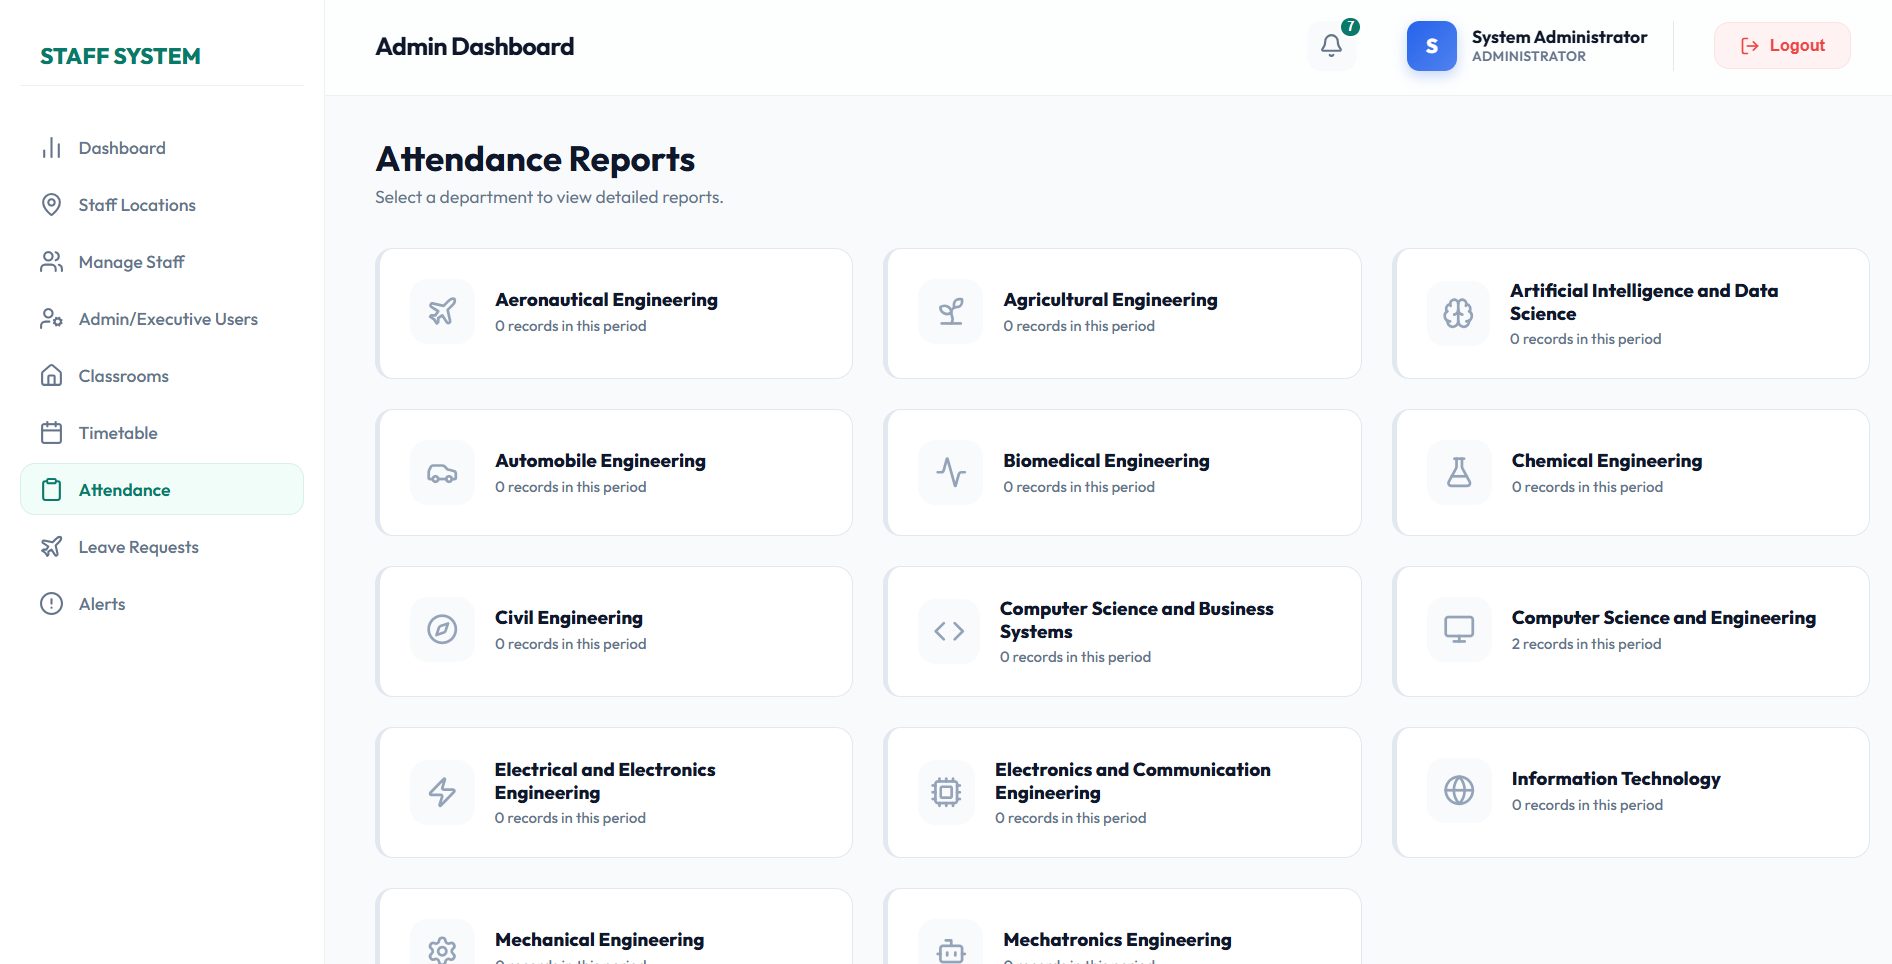
\includegraphics[width=0.8\textwidth]{images/reports_view.png}
\caption{Automated Attendance Reports and Historical Logs Interface}
\end{figure}

\section{Substitution and Meeting Requests Interface}
Special high-level roles (like the Principal or Secretary) have an exclusive interface to call staff for emergency meetings. When invoked, the system checks if the target staff has an ongoing class. If so, it automatically queries the database backend for currently available (free) staff and dispatches an immediate web push notification and email to request a substitution cover.

\begin{figure}[H]
\centering
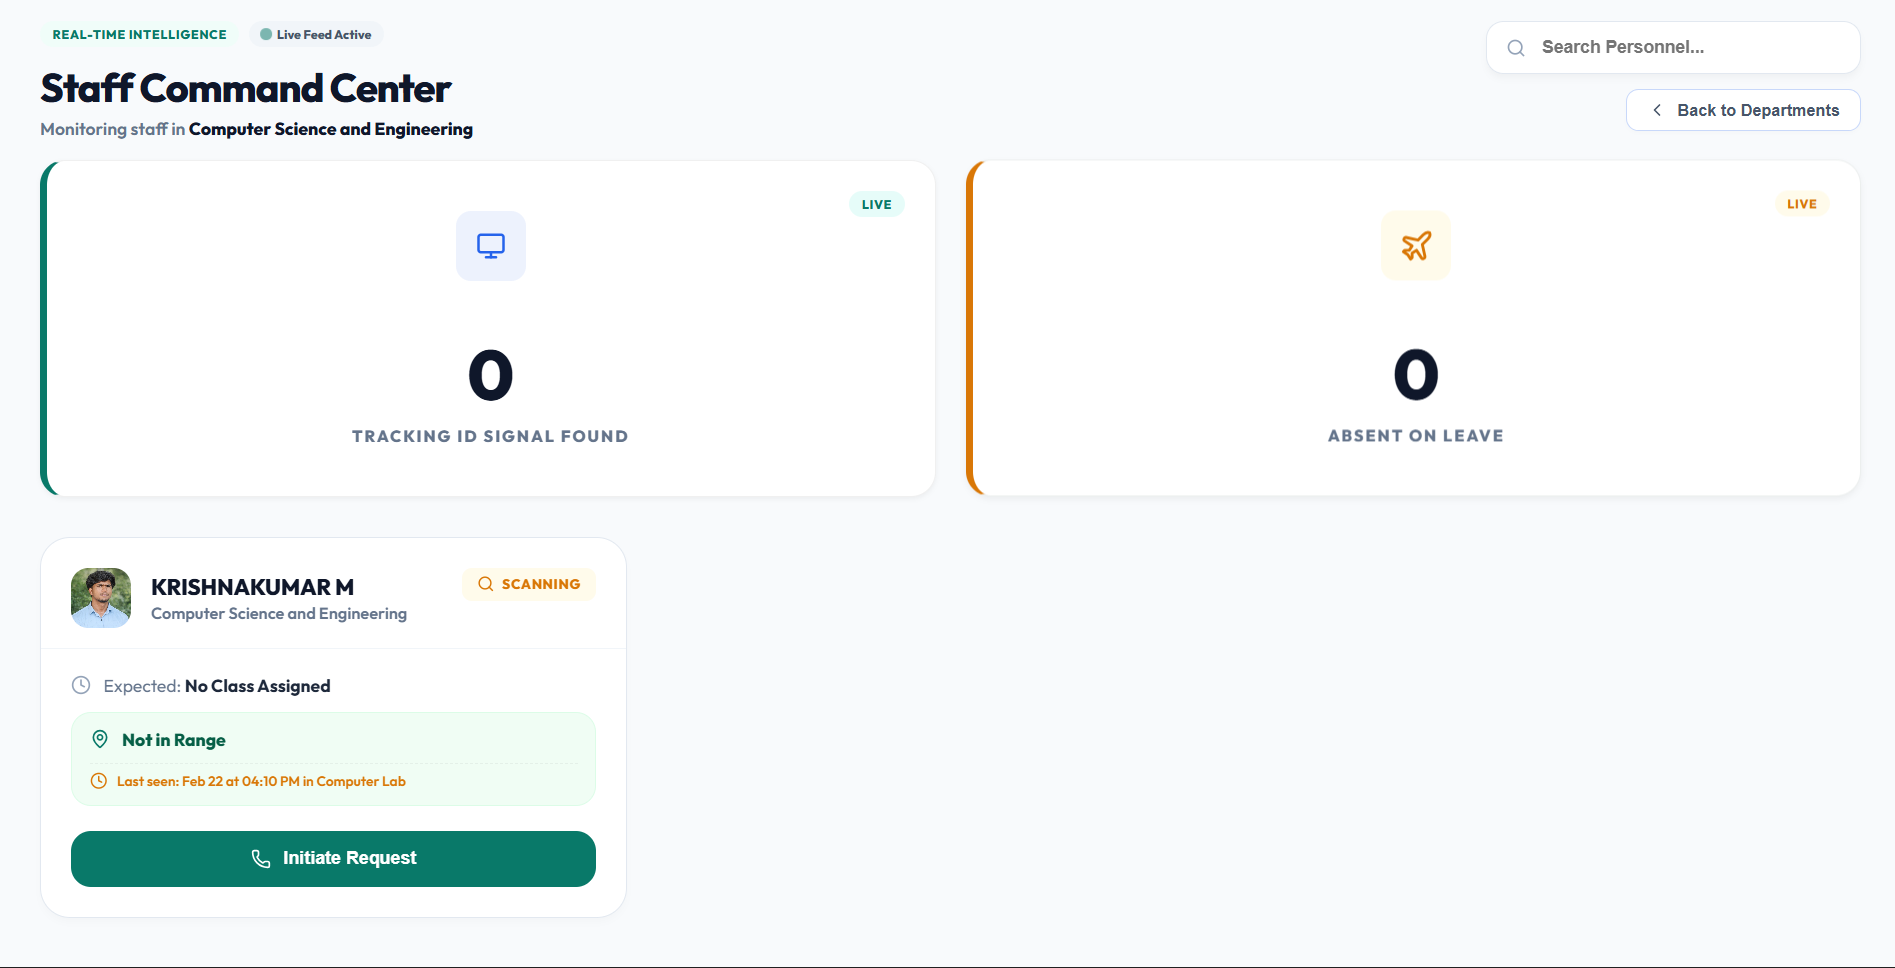
\includegraphics[width=0.8\textwidth]{images/substitution_requests.png}
\caption{Meeting and Automated Substitution Handling Interface}
\end{figure}
